 \documentclass{report}
 
\usepackage[utf8]{inputenc} 
\usepackage[T1]{fontenc}      
\usepackage[top=2.0cm, bottom=3cm, left=3.0cm, right=3.0cm]{geometry}
\usepackage{graphicx}
\usepackage{wrapfig}
\usepackage{amsmath,esint }
\usepackage{amssymb}
\graphicspath{{figures/}{../figures}}

\newcommand*\dif{\mathop{}\!\mathrm{d}}
\newcommand*\diver{\mathop{}\!\mathrm{div}}
\newcommand*\grad{\mathop{}\!\mathrm{grad}}

\begin{document}

\section*{Le Petit Prince : satellisation d'une pomme}

On se place à la surface d'une planète de rayon $R$ et de champ gravitationnel $g$. On envoie une pomme avec une vitesse $v_0$ purement horizontale et on négligera les frottements de l'air.

\begin{itemize}
\item En supposant la planète localement plane, déterminer la hauteur d$z$ dont est tombée la pomme après avoir parcouru une longueur d$x$ dans le plan horizontal. % d$z=\dfrac{g(\mathrm{d}x)^2}{2{v_0}^2}$
\item Après une distance horizontale d$x$, de combien le sol de la planète est-il descendu ? On pourra utiliser les formules pour les petits angles : $\tan\theta\simeq \theta$, $\sin\theta\simeq \theta$ et $\cos\theta\simeq 1-\theta^2/2$. % Il faut penser à la rotondité de la Terre qui n'est donc pas parfaitement plane localement : d$h=R-R\cos(\mathrm{d}\theta)=R(\mathrm{d}\theta)^2/2=(\mathrm{d}x)^2/2R$
\item En déduire qu'il existe une certaine vitesse $v_0$ pour laquelle la pomme va revenir à son point de départ. % v_0=\sqrt{GM/R}$
\end{itemize}

\newpage

\section*{Projectile lancé à la verticale}

On tire un petit projectile à la verticale, avec une vitesse initiale $v_0$. Le problème est de calculer son altitude $z$ en fonction du temps, en tenant compte de la gravité et de la résistance de l'air. Comme l'objet est petit, on supposera que la résistance de l'air est proportionnelle à la vitesse et que la force de résistance est $m\gamma v$, $m$ étant la masse de l'objet, $v$ sa vitesse et $\gamma$ une constante. Nous supposerons que la force de gravité est constante (on néglige sa variation en fonction de l'altitude). On adoptera comme origine la position du tir ($z=0$) et on supposera que le mouvement ne se produit que dans la direction $z$.

\begin{itemize}
\item Soit $v(t)$ la composante en $z$ de la vitesse du projectile. \'{E}crivez l'équation différentielle que doit satisfaire $v(t)$ en fonction du temps, d'après la deuxième loi de Newton.
\item Résoudre cette équation différentielle avec la condition initiale $v(0)=v_0$.
\item Exprimer maintenant l'altitude $z$ en fonction du temps.
\item Calculer l'altitude maximale atteinte par le projectile ($z_\mathrm{max}$), en fonction des paramètres $v_0$, $g$ et $\gamma$.
\item Exprimer le résultat de la question précédente ($z_\mathrm{max}$) dans les limites de très faible résistance ($\gamma \rightarrow 0$) et de très forte résistance ($\gamma \rightarrow \infty$). Quelles modifications mineures devrait-on apporter à l'équation différentielle trouvée première question pour retrouver ces résultats plus simplement ?

\end{itemize}

\newpage

\section*{Paramètre d'impact}

Une météorite arrive depuis l'infini vers la Terre avec une vitesse à l'infini $\vec{v}_0$. La Terre a une masse $M_T$ et un rayon $R_T$. On note $b$ le paramètre d'impact comme indiqué sur la figure ci-dessous. L'objectif de ce problème est de déterminer la valeur minimale de $b$ pour laquelle la météorite évite la collision avec la Terre.

\begin{figure}[h]
\centering
  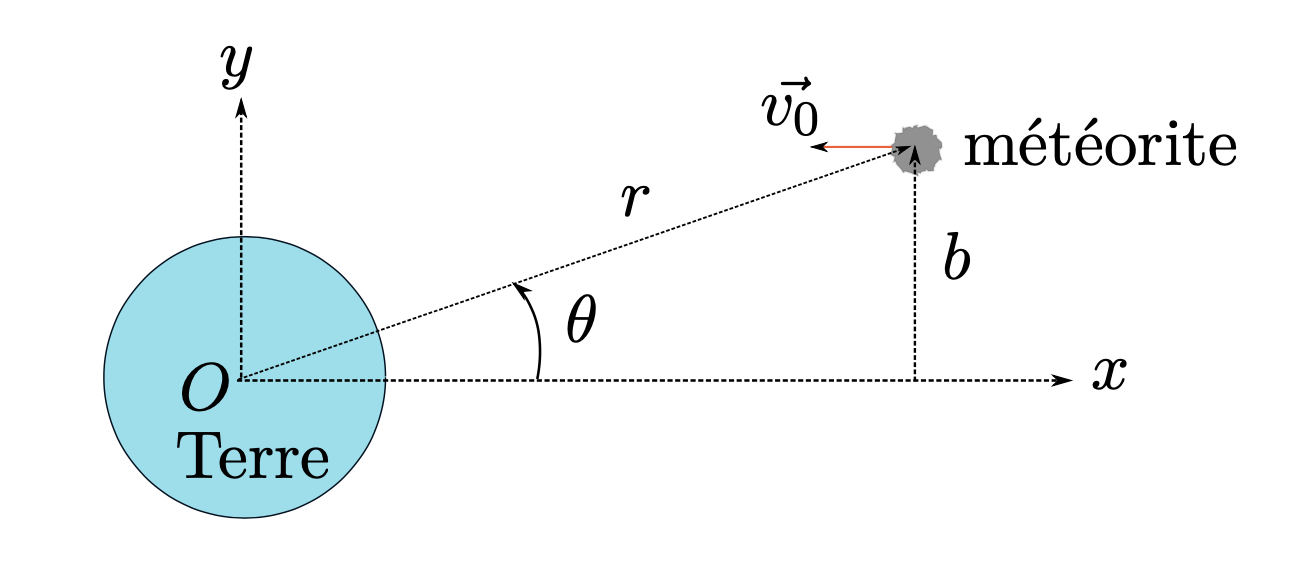
\includegraphics[scale=0.4]{parametre_impact.png}
\end{figure}

\begin{itemize}
\item La météorite n'est soumise qu'à la force gravitationnelle de la Terre. Déterminer la nature de sa trajectoire. Montrer que le mouvement est plan et déterminer une relation entre $r$ et $\dot{\theta}$.
\item On note $N$ le point de la trajectoire où la distance qui sépare la météorite de la Terre est la plus petite. Montrer qu'en $N$, la vitesse est uniquement suivant $\vec{u}_\theta$. Déterminer une relation entre $v_N$ au point $N$, la distance $ON$, $b$ et $v_0$.
\item En utilisant la conservation de l'énergie, montrer la relation :
$$
0=r^2_\mathrm{min}v_0^2+2GM_Tr_\mathrm{min}-v_0^2b^2.
$$
\item En déduire l'expression minimale $b_c$ du paramètre d'impact telle que pour $b<b_c$, la météorite frappe la Terre et pour $b>b_c$, la météorite évite la Terre. On pourra exprimer le résultat en fonction de la vitesse de libération $v_\mathrm{lib}$.
\end{itemize}

\newpage

\section*{Piège de Penning}

A l'aide d'un dispositif approprié, on créé dans une région de l'espace au voisinage d'un point $O$ un champ électrique défini en coordonnées carthésiennes par :
\begin{align*}
	\vec{E}=\frac{U_0}{2R^2}\left(-x\vec{e}_x-y\vec{e}_y+2z\vec{e}_z \right) 
\end{align*}
Un électron de masse $m$ et de charge $e$ se meut dans la région située autour du point $O$.
\begin{itemize}

	\item[$\ominus$] Montrer que le point $O$ est une position d'équilibre pour l'éléctron. Discuter de la stabilité selon les directions. On introduira $\omega_z^2=eU_0/mR^2$.
	
\end{itemize}

Pour stabiliser la trajectoire de l'électron, on supperpose au champ électrique un champ magnétique uniforme et constant $\vec{B}=B_0\vec{e}_z$. On définit $\omega_c=eB_0/m$. 

\begin{itemize}

		\item[$\ominus$] Montrer que le mouvement suivant $\vec{e}_z$ est inchangé.
		
		\item[$\ominus$] Pour le mouvement dans le plan $(xOy)$, montrer que l'électron n'est piégé que si $B_0$ est supérieur a une certaine valeur $B_c$, à déterminer en fonction des données de l'exercice. On utilisera le changement de variable : $\rho = x+iy$.
		
		\item[$\ominus$] Résoudre l'équation en $\rho$ pour le cas $B_0\gg B_c$, sans chercher à mettre en évidence les constante d'intégration, mais en mettant en évidence deux pulsations, l'une voisine de $\omega_c$, notée $\omega_c'$, et une autre notée $\omega_m$, appelée pulsation magnétique. 
		
\end{itemize}

\newpage

\section*{Tir à grande distance}

Dans le jeu \textit{Call of Duty 4 : Modern Warfare}, le joueur prend le rôle d'un tireur d'élite devant abattre une cible située à une distance $d=$897m à l'aide d'un fusil de précision, qui tire un projectile à une vitesse $v_0=850$m.s$^{-1}$. Le tir s'effectue depuis le dernier étage d'un immeuble d'une hauteur $H=30$m, la cible se trouvant plein nord par rapport au tireur. La scène se situe en Russie, à une latitude $\lambda=45^\circ$. Le coéquipier du joueur précise, avant le tir, qu'il faut tenir compte de l'effet de Coriolis et l'on souhaite vérifier cette affirmation.

On définit $R=(O,x,y,z)$ le repère situé au pied de l'immeuble où se trouve le joueur, avec l'axe $\vec{e}_x$ dirigé vers l'est et l'axe $\vec{e}_y$ se dirigeant vers le nord. On notera $\vec{\Omega}_T$ le vecteur rotation de la terre. On supposera que les frottements de l'air sont négligés.

\begin{itemize}

	\item[$\dagger$] Ecrire les équations du mouvement dans le référentiel $R$ de la balle une fois que le tireur fait feu.
	
	\item[$\dagger$] Déterminer la solution sur $x(t)$ sans préciser les variables d'intégration.
	
	\item[$\dagger$] Donner une estimation du temps de vol avant impact $t_{impact}$ puis simplifier les équations du mouvement, les résoudre.
	
	\item[$\dagger$] Que pensez-vous de l'affirmation du coéquipier ? Quel est l'écart $\vec{\varepsilon}$ de la balle par rapport à si celle-ci avait une trajectoire parfaitement rectiligne ?

\end{itemize}

\end{document}